\section{Approach}

% draw two pics, one is overview, describing a detail example. from candidate generation, focus entity identification, and a basic siamese structure. The other one is detailed network structure of our schema encoding.
In this section, we describe our nerual network based model for KBQA. The architecture of our proposed model is shown in \figref{fig:overview}. First, we identify focus entity and generate candidate query graphs by searching paths with certain constraints in KB (\secref{sec:candgen}). Next we encode question and candidate query graph respectively. 
More specifically, we use a bi-directianl RNN structure to represent question (\secref{sec:q-encoding}) and a complex embedding strategy is employed to encode a complex query graph (\secref{sec:schema-encoding}). Then we propose a cross attention mechanism to measure the similarity between a question and a query graph (\secref{sec:attention}). Finally, we discuss the prediction and parameter learning step of this task (\secref{sec:training}).


\begin{figure*}
	\centering
	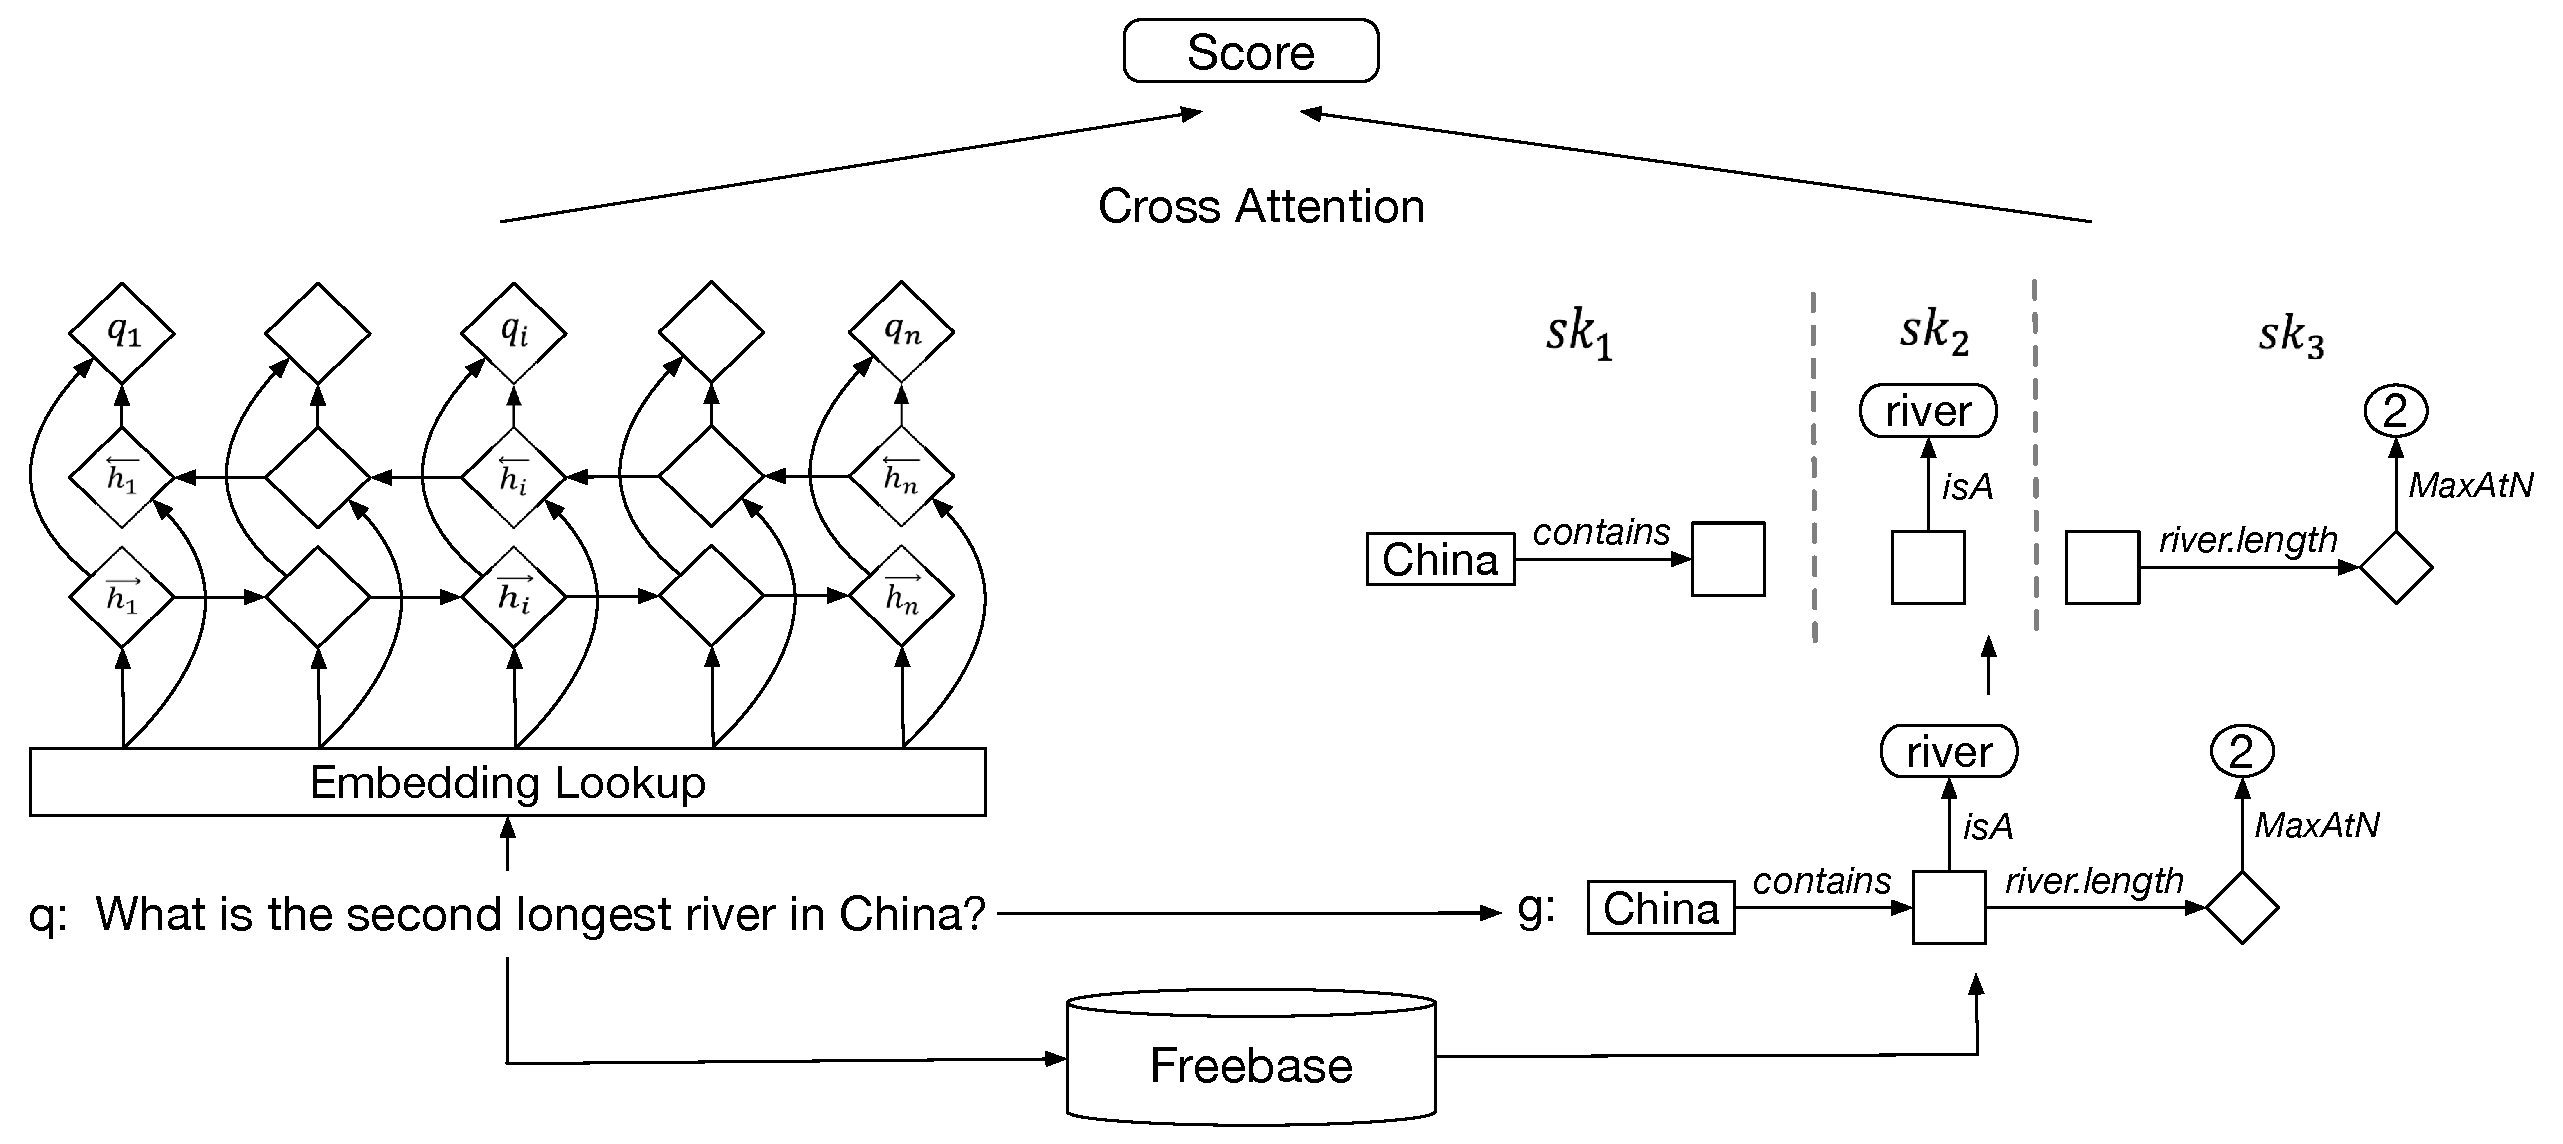
\epsfig{file=figures/overview.eps, angle=0, width=2.0\columnwidth}
	%\scalebox{0.3}{\includegraphics{overview.eps}}
	\caption{Overview of proposed neural network model.}
	\label{fig:overview}
\end{figure*}


\subsection{Candidate Generation}
\label{sec:candgen}

Given a question, we have to generate a set of query graphs with multiple complex constraints. There are four different constraints which are entity constraint, type constraint, temporal constraint and ordinal constraint. 





\subsection{Question Representation}
\label{sec:q-encoding}

We use Bi-GRUs to encode the question. Firstly we introduce RNNs and GRUs which are frequently mentioned when encoding sequential data. Then we descirbe how to encode the question using Bi-GRUs in our model.

RNNs are a f amily of neural networks designed for sequential data and have shown great promise in many NLP tasks. RNNs take a sequence of vectors $(\bi{x}_1, \bi{x}_2, \dots, \bi{x}_n)$ and return another sequence $(\bi{h}_1, \bi{h}_2, \dots, \bi{h}_n)$ that represents the hidden state information about the sequence at each time step in the input. In theory, RNNs can learn long dependencies but in practice they seem to be biased towards their most recent inputs of the sequence. Thus GRUs and LSTMs are proposed and they have shown great capabilities to capture long-range dependencies. We describe GRUs which is used in our model in detail.

As shown in \figref{fig:gru}, the hidden state $\bi{h}_t$ at current time step $t$ of GRUs is computed by interpolating between the hidden state $\bi{h}_{t-1}$ at previous time step and the candidate state $\tilde{\bi{h}}_t$.

\begin{equation}
\label{eqn:gru1}
\begin{aligned}
& \bi{h}_t & = & (1-\bi{z}_t)\cdot\bi{h}_{t-1}+\bi{z}_t\cdot\tilde{\bi{h}}_t\\
\end{aligned}
\end{equation}
\noindent
where $\bi{z}_t$ is the update gate and $\cdot$ is the element-wise vector product.

The update gate $\bi{z}_t$ for the interpolation is computed from the current input vector $\bi{x}_t$ and the previous hidden state $\bi{h}_{t-1}$ at time step $t-1$.

\begin{equation}
\label{eqn:gru2}
\begin{aligned}
& \bi{z}_t & = & \sigma(\bi{W}_z\bi{x}_t+\bi{U}_z\bi{h}_{t-1})\\
\end{aligned}
\end{equation}
\noindent
where $\bi{W}_z$ and $\bi{U}_z$ are model parameters to be learned during training and $\sigma$ is the sigmoid activation function which is a element-wise operation on the vectors.

\begin{equation}
\label{eqn:gru3}
\begin{aligned}
& \sigma(\bi{x}) & = & 1/(1+e^{-\bi{x}})\\
\end{aligned}
\end{equation}
\noindent

The candidate state $\tilde{\bi{h}}_t$ at current time step is computed using the current input $\bi{x}_t$ and the previous state $\bi{h}_{t-1}$ at time step $t-1$.

\begin{equation}
\label{eqn:gru4}
\begin{aligned}
& \tilde{\bi{h}}_t & = &\mbox{tanh}(\bi{W}_h\bi{x}_t+\bi{U}_h(\bi{r}_t\cdot\bi{h}_{t-1}))\\
\end{aligned}
\end{equation}
\noindent
where $\bi{W}_h$ and $\bi{U}_h$ are model parameters to be learned during training and $\mbox{tanh}$ is the hyperbolic tangent activation function and $\bi{r}_t$ is the reset gate, computed as follows,

\begin{equation}
\label{eqn:gru5}
\begin{aligned}
& \bi{r}_t & = & \sigma(\bi{W}_r\bi{x}_t+\bi{U}_r\bi{h}_{t-1})\\
\end{aligned}
\end{equation}
\noindent
where $\bi{W}_r$ and $\bi{U}_r$ are parameter matrics to be learned.

The advantage of using gated units such as GRU or long short-term memory (LSTM) is their ability to process infomation of longer sequences. In the case of the GRU, the reset gate $\bi{r}_t$ determines which parts of the previous state $\bi{h}_{t-1}$ are ``ignored'' in the computation of the candidate state and the update gate $\bi{z}_t$ determines how much of the previous state is ``leaked'' into the current state $\bi{h}_t$. The update gate could decide to forget the previous state altogether or to simply copy the previous state and ignore the current input. Both gates are parameterized (and thus trainable) and their values depend on both the input $\bi{x}_t$ and the previous state $\bi{h}_{t-1}$.

To encode the question, we have to obtain the representation of each word of the question. Suppose question $q$ is expressed as $q=(x_1, x_2, \dots, x_n)$, where $x_i$ denotes $i$th word. We first look up a word embedding matrix $E_x\in \mathbb{R}^{d\times v}$to get the word embeddings $\bi{q}=(\bi{x}_1, \bi{x}_2, \dots, \bi{x}_n)$, which is initialized by pre-train word embedding tools such as Word2vec, and update during the training process. Here, $d$ denotes the dimension of the embeddings and $v$ denots the vocabulary size of natural language words.

Then, the embeddings are fed into a bidirectional GRU networks. If we use unidirectional GRU, the outcome of current word is based on only the words before it so the infomation of the words after it is totally lost. To avoid this, we use bi-GRU which consists a forward network handles the question from left to right and a backward network do in the reverse order. Therefore, we get two hidden state sequences, $(\overrightarrow{\bi{h}_1}, \overrightarrow{\bi{h}_2}, \dots, \overrightarrow{\bi{h}_n})$ from forward network and $(\overleftarrow{\bi{h}_1}, \overleftarrow{\bi{h}_2}, \dots, \overleftarrow{\bi{h}_n})$ from backward network. We concatnate the forward hidden state of each word with corresponding backward hidden state, resulting in a representation $[\overrightarrow{\bi{h}_i};\overleftarrow{\bi{h}_i}]$ ($\bi{q}_i$). Thus, we obtain the representation of each word in the question.


\subsection{Query Graph Representation}
\label{sec:schema-encoding}

After candidate generation, we obtain a set of candidate complex query graphs for each question $q$. A complex query graph $g$ can be regarded as a set of simple skeletons $(sk_1, sk_2, \dots, sk_m)$. We define a skeleton $sk$ is a predicate path starting from a fixed node to the target answer. The fixed starting node can be an entity, a type, a number, datetime or an ordinal value. Together with predicate, we call them ``items''. Thus we denote $sk = (it_1, it_2, \dots, it_l)$ (Note that this sequence has an order from starting point to target answer). In the case of \figref{fig:overview}, the candidate query graph in the right side can be splited into three skeletons, which start from ``entity:China'', ``type:River'' and ``ordinal$\_$value:$2$'' respectively. 
Now we describe in detail how to obtain the skeleton representation $\bi{sk}$ and further represent a complex query graph $g$ into $\bi{g} = (\bi{sk}_1, \bi{sk}_2, \dots, \bi{sk}_m)$. 

%1. item encoding
Firstly, we represent each component (item) of a skeleton into hidden vectors. For entity, type and predicate, we use their names in KB as text infomation and thus employ a bi-GRU network to encode the items just as we do in question encoding (\secref{sec:q-encoding}). For example, the name of entity ``China'' in \figref{fig:overview} is \textit{``People's Republic of China''} and we regard it as a word sequence [``people'', ``republic'', ``of'', ``China'']. After embedding lookup, the sequence of word embeddings are fed into bi-GRU, resulting a sequence of hidden vectors $[\overrightarrow{\bi{h}_i};\overleftarrow{\bi{h}_i}]$. Then we average them to obtain the item representation $\bi{it}$.

\begin{equation}
\label{eqn:item}
\begin{aligned}
& \bi{it} & = & \frac{1}{N}\sum_{i}[\overrightarrow{\bi{h}_i};\overleftarrow{\bi{h}_i}]\\
\end{aligned}
\end{equation}
\noindent
where $N$ is the number of words in that name.
For number, datetime and ordinal value, we add three special placeholders in word embedding vocabulary and initialize them randomly. Thus, these three items are represented directly through embedding lookup. 

%2. skeleton representation

Then, we represent a skeleton $\bi{sk}$ as a dynamic combination of its item representations $\bi{it}_i$ shown in \figref{fig:overview} (right side). Since the items of a skeleton also form into a sequence in order, we use another bi-GRU to encode item sequence.

Up to now, we have obtained the representation of query graph $\bi{g}$ consisting of a set of skeletion representations $(\bi{sk}_1, \bi{sk}_2, \dots, \bi{sk}_m)$.




\subsection{Attention Mechanism}
\label{sec:attention}

Attention mechanisms \cite{bahdanau2014neural,luong2015effective} have become an integral part of sequence modeling and transduction models in various nlp tasks, allowing better understanding sequential data. In this paper, we introduce a cross-attention mechanism between question and query graph, aiming to better justify thier compatibility.

Our cross-attention mechanism consists of two parts: query graph towards question part and question towards query graph part. Our goal is to find the best query graph from the candidate set. When we look at a question $\bi{q} = (\bi{q}_1, \bi{q}_2, \dots, \bi{q}_n)$ and a candidate query graph $\bi{g} = (\bi{sk}_1, \bi{sk}_2, \dots, \bi{sk}_m)$, we have to judge which parts of the query graph are more related to the question, since each skeleton of a graph describes one semantic aspect of the question. Besides, when we look at the query graph, we will reread the question to find out which words are more focused. Hao et al., \cite{hao2017end} also propose a cross-attention mechanism, aiming to select the best answer towards a question. However, their method does not calculate the attention values on both sides simultaneously, instead they do it in two steps and use an average of word representations in question to guide the attention of answer aspects. 

\begin{figure*}
	\centering
	\epsfig{file=figures/attention.eps, angle=0, width=1.2\columnwidth}
	%\scalebox{0.5}{\includegraphics{figures/attention.eps}}
	\caption{Cross-attention architecture between question and query graph.}
	\label{fig:attention}
\end{figure*}

Inspired by ABCNN \cite{yin2015abcnn}, we propose a attention matrix $\bi{E}_{att}$  (\figref{fig:attention}), where the attention values of row $i$ denote the attention distribution of the $i$-th word in the question with respect to the query graph, and the attention values of column $j$ denote the attention distribution of the $j$-th skeleton in the query graph with respect to the question. Then we represents the whole question $\bi{q}$ and query graph $\bi{g}$ as follows. 




\begin{equation}
\label{eqn:att-q}
\begin{aligned}
& \bi{q} & = & \sum_{i}(\sum_{j}{\bi{E}_{att}}_{ij}) \times \bi{q}_i\\
\end{aligned}
\end{equation}
\noindent

\begin{equation}
\label{eqn:att-g}
\begin{aligned}
& \bi{g} & = & \sum_{j}(\sum_{i}{\bi{E}_{att}}_{ij}) \times \bi{sk}_j\\
\end{aligned}
\end{equation}
\noindent

In the end, we use a fully connected layer to get a similarity score between $\bi{q}$ and $\bi{g}$.



\subsection{Training and Prediction}
\label{sec:training}






